\documentclass[11pt]{article}

\usepackage{amsmath}
\usepackage{amssymb}
\usepackage{graphicx}
\usepackage{booktabs}
\usepackage[margin=1in]{geometry}
\usepackage{tikz}
\usepackage{pgfplots}
\pgfplotsset{compat=1.18}
\usetikzlibrary{arrows.meta,positioning,shapes.geometric}
\usepackage[colorlinks=true,linkcolor=black,citecolor=black,urlcolor=blue]{hyperref}

\newcommand{\Voc}{V_{\mathrm{OC}}}
\newcommand{\Vocrad}{V_{\mathrm{OC,rad}}}
\newcommand{\mV}{\,\mathrm{mV}}

\title{A Two-Measurement Reduction of the Non-Contact Implied-$\Voc$ Protocol}

\author{Gyalpo Dongo \and Sebastian Alberdi}
\date{August 2026}

\begin{document}
\maketitle

\begin{abstract}
The non-contact implied open-circuit voltage ($\Voc$) protocol of Louks \emph{et al.}~\cite{louks2025} infers a solar absorber's radiative-limit voltage from three optical measurements, namely steady-state photoluminescence (SRPL), time-resolved photoluminescence (TRPL), and optical transmission, fed to a detailed-balance model. We ask a pure \emph{information-sufficiency} question: does there exist a reduced protocol using at most two of the three modalities, at a strictly smaller acquisition budget (measurement time and integrated photon dose), that reproduces the full protocol's \emph{own} implied $\Voc$ to within 10~mV worst-case, leave-one-device-out across a synthetic grid of realistic p--i--n stacks under certification measurement noise? A sealed, deterministic verifier is the sole oracle; the search only edits candidate protocol dicts. We enumerate exhaustively every \emph{single-config-per-modality} protocol of at most two modalities under a smaller budget (a finite set) and treat multi-config repeats, which the contract also admits (buying precision as $\sqrt{\text{dose}}$), separately by argument. \textbf{Result: the reduction exists.} The protocol $\{$SRPL, transmission$\}$, obtained by dropping TRPL, passes and is the only two-modality subset containing a passer; the cheapest certified passer (SRPL at fluence $0.25$~suns, $50$~ms window; transmission at $20$~ms) recovers the full implied $\Voc$ to $9.13\mV$ worst-case at $68\%$ less acquisition time and $93\%$ less photon dose than the three-measurement protocol. The result is simultaneously a certified partial negative: TRPL is non-load-bearing for the implied-$\Voc$ scalar \emph{by construction} (setup leverage $0.31\mV$), whereas SRPL ($20.06\mV$) and transmission ($47.25\mV$) are load-bearing, and every enumerated single-config protocol that drops either fails the bar. Dropping transmission cannot be rescued by any amount of PL repetition (PL carries no absorption-edge or thickness information); dropping SRPL floors at $20.06\mV$ for single configs, and we scope the negative accordingly rather than claiming multi-config TRPL repeats were graded. Scope is strictly the pinned model's own implied $\Voc$; the ${\sim}170\mV$ real-device stack offset reported in~\cite{louks2025} is out of scope. All numbers are sealed-verifier verdicts.
\end{abstract}

\section{Introduction}

Measuring a solar absorber's voltage potential without fabricating a full contacted device is valuable: it lets a materials team rank stacks and diagnose losses early, before electrodes and interfaces confound the measurement. The \emph{implied} open-circuit voltage $\Voc$ is the standard non-contact proxy. It is the quasi-Fermi-level splitting a photoexcited absorber would sustain, and it factors into a radiative-limit term set by the absorption edge and a recombination penalty set by the photoluminescence quantum efficiency (PLQE):
\begin{equation}
\Voc \;=\; \Vocrad(E_g, E_U, d)\;-\;kT\,\bigl|\ln \mathrm{PLQE}\bigr|,
\label{eq:voc}
\end{equation}
where $E_g$ is the bandgap, $E_U$ the Urbach energy (band-edge disorder), $d$ the absorber thickness, and $kT$ the thermal voltage~\cite{ross1967,rau2007}. The radiative term $\Vocrad$ follows from detailed balance~\cite{shockleyqueisser1961}: an Urbach-broadened absorptance edge~\cite{urbach1953} integrated against a Boltzmann emission tail gives the radiative saturation current, and against a fixed solar spectrum gives the absorbed generation current.

The published protocol of Louks \emph{et al.}~\cite{louks2025} obtains the three inputs to Eq.~\eqref{eq:voc} from three separate optical measurements: \emph{transmission} gives the absorption edge ($E_g$), the thickness ($d$), and a route to $E_U$; \emph{steady-state PL} (SRPL) gives PLQE directly plus a second route to $E_U$; and \emph{time-resolved PL} (TRPL) gives PLQE indirectly through a kinetic reconstruction of the non-radiative rate. Three measurements cost acquisition time and photon dose. A natural question for anyone deploying the protocol at scale is whether all three are actually necessary to pin the implied-$\Voc$ number, or whether a cheaper subset carries the same information.

This paper answers that question for one pinned forward model. We stress at the outset what is and is not being asked. This is an \textbf{information-sufficiency} question about the model's \emph{own} output: can a reduced measurement set reproduce, to $10\mV$, the implied $\Voc$ that the full three-measurement pipeline computes for the same device? It is \emph{not} a claim that either protocol matches a device's measured current--voltage $\Voc$. Real perovskite p--i--n stacks carry a ${\sim}170\mV$ offset between implied and contacted $\Voc$ from transport and interface losses~\cite{louks2025}; that offset is identical for the full and reduced protocols (both target the same model output) and is explicitly out of scope here.

\paragraph{Contribution.} Working under a single pinned forward model and a sealed deterministic verifier, we (i) enumerate exhaustively every \emph{single-config-per-modality} measurement protocol of at most two modalities whose acquisition budget strictly dominates the full protocol's; (ii) certify that exactly one subset ($\{$SRPL, transmission$\}$) contains passers, exhibit three of them, and report the cheapest; and (iii) certify the complementary negative over that single-config space (every SRPL-dropping or transmission-dropping single-config protocol fails, with a quantified near-miss frontier) and give the budget-and-precision argument that bounds what multi-config repeats (which we did not exhaustively grade) could and could not rescue. The honest one-line headline: \emph{for this model's implied $\Voc$, TRPL is redundant and the other two measurements are each load-bearing.}

\section{Methods}

\subsection{The forward model and the reduction target}
\label{sec:forward}

A single pinned forward model (frozen inside the verifier) defines both the ground truth and the candidate outputs. For a device with parameters $(E_g, E_U, d, \mathrm{PLQE})$, the radiative term $\Vocrad$ is computed by detailed balance: with an above-gap absorption coefficient $\alpha_0=10^5\,\mathrm{cm}^{-1}$ and an Urbach tail $\alpha(E)=\alpha_0\exp[(E-E_g)/E_U]$ below the gap, the thickness-dependent absorptance $a(E)=1-e^{-\alpha(E)d}$ is integrated against a Boltzmann emission tail (giving $J_{0,\mathrm{rad}}$) and against a fixed solar generation spectrum (giving $J_{\mathrm{sc}}$), so that $\Vocrad = kT\ln(J_{\mathrm{sc}}/J_{0,\mathrm{rad}})$. The recombination penalty is $kT\,|\ln\mathrm{PLQE}|$ as in Eq.~\eqref{eq:voc}.

The \emph{reduction target} is not an absolute truth but the full protocol's own noisy output. Ground truth for grading is the FULL three-measurement protocol's implied $\Voc$ on the same device and noise seed, so that any modality retained by both the full and reduced protocols carries \emph{identical} noise draws; the graded difference is therefore exactly the information the dropped modality would have contributed, nothing else.

\subsection{Measurement map and noise model}

Each modality maps to native quantities with shot-noise-limited precision, the $1\sigma$ level scaling as $\sqrt{d_{\mathrm{nom}}/d_{\mathrm{act}}}$ (nominal over actual dose; repeats and longer windows buy precision, and the budget charges for them):
\begin{itemize}
\item \textbf{Transmission} $\rightarrow$ bandgap $E_g$ ($\pm 2\mV$ nominal), thickness $d$, and Urbach $E_U$.
\item \textbf{SRPL} $\rightarrow$ PLQE \emph{directly} (log-space $\sigma=0.03$ nominal; precise) and a second route to $E_U$.
\item \textbf{TRPL} $\rightarrow$ PLQE \emph{indirectly} through the kinetic model (log-space $\sigma=0.20$ nominal; unbiased but ${\sim}7\times$ less precise, as it assumes injection level and radiative coefficient).
\end{itemize}
When both PLQE routes are present, the full protocol fuses them by inverse-variance weighting. A reduced protocol that drops a modality sees \emph{only} the retained modalities' simulated data plus protocol-independent, leave-one-device-out (LODO) population priors for any dropped quantity, it never sees a full-protocol intermediate or the dropped measurement's derived quantity. This is the integrity firewall that makes the question about information, not leakage. Crucially, no PL measurement (SRPL or TRPL, at any dose) produces an estimate of $E_g$ or $d$: those come only from transmission or, when transmission is dropped, from the LODO priors.

\subsection{Search space and the acquisition budget}
\label{sec:space}

A candidate is a protocol dict $\{$\texttt{modalities}: subset of size 1--2; \texttt{configs}: per-modality $(\text{fluence}\times\text{window})$ settings from a pinned menu$\}$. A modality may carry \emph{multiple} configs (repeats/averaging), which lowers that modality's measurement noise as $\sqrt{\text{dose}}$ at a proportional budget cost. The budget is a pair (total time in ms, total integrated photon dose) computed by a pinned accounting. The pinned \emph{full} protocol is SRPL$(1.0\,\text{suns},100\,\text{ms})$ + TRPL$(1.0,100\,\text{ns})$ + transmission$(20\,\text{ms})$, with budget $(\text{time},\text{dose})=(220, 201)$. There are six non-empty subsets of size $\le 2$.

\paragraph{What we enumerate, and what we argue.} The single-config-per-modality space (one $(\text{fluence}\times\text{window})$ choice on each retained modality) is small and we enumerate it \emph{exhaustively}: search run~1 explored $229$ candidates and run~2 explored $161$ (candidates rejected on the well-formedness or budget gates included). The contract additionally admits \emph{multi-config} (repeat) protocols, and we did \emph{not} brute-force those; we treat them by a budget-and-precision argument (\S\ref{sec:negative}). This distinction is material only for the negative result, and only for the SRPL-dropping family, as we make precise there; the positive result and the transmission-dropping negative are unaffected by repeats.

\subsection{Gates (the verdict)}

The sealed verifier returns \texttt{valid:True} iff all gates pass:
\begin{itemize}
\item \textbf{G2 (well-formed):} 1--2 modalities, every config on the pinned menu.
\item \textbf{G3 (strictly smaller budget):} the candidate's $(\text{time},\text{dose})$ must Pareto-dominate $(220,201)$, both no larger, at least one strictly smaller.
\item \textbf{G1 (recovery):} worst-case over $24$ pinned devices $\times$ $20$ certification seeds (\texttt{CERT\_SEEDS}$=1000\ldots1019$, a namespace disjoint by construction from any screening seeds) of $\bigl|\,\Voc^{\mathrm{reduced}} - \Voc^{\mathrm{full}}\,\bigr| \le 10\mV$ (both implied), leave-one-device-out.
\item \textbf{G4 (determinism):} \texttt{verify} is a seeded deterministic function; the engine double-runs every claimed hit and requires byte-identical verdicts.
\end{itemize}

\subsection{Harness protocol (pre-registration, blinded oracle, ratchet)}
\label{sec:harness}

The campaign ran inside an autoresearch harness whose non-negotiables gate what may enter the ledger. (1) \emph{Pre-registration:} the public contract (objective, search space, budget accounting, and all four gates) was frozen before any candidate was graded, and its SHA (which hashes \texttt{CONTRACT.md}) is recorded in every ledger entry and is constant across the campaign. (2) \emph{Blinded oracle:} the searcher never sees the verifier's battery; it emits candidate dicts and reads only \texttt{valid:True/False}. It may not read certification seeds, may not tune to them, and may not touch the verifier or forward model, an integrity violation taints the whole line of work. (3) \emph{Ratchet:} only a sealed-verifier \texttt{valid:True} verdict is a hit; nothing self-reported enters the ledger. (4) \emph{Refutations held higher than wins:} a claimed hit is accepted only after a byte-identical double-run. Two setup-time self-checks guard the referee itself: a \emph{dress rehearsal} requires the full pipeline to reproduce the true implied $\Voc$ at infinite dose to $<10^{-6}\,\mathrm{V}$ (else \texttt{verify} raises \textsc{inconclusive} rather than scoring), and \emph{pre-search checks} report the full-protocol seed scatter (an ill-posed-bar kill if it already exceeds $10\mV$) and each modality's leverage. We note that the \emph{contract} SHA pins the public contract text, not the oracle source: the verifier code itself received reviewer patches after the freeze (\S\ref{sec:integrity}); the contract, the grid, and the gates were never changed. Figure~\ref{fig:loop} shows the loop for this campaign.

\begin{figure}[t]
\centering
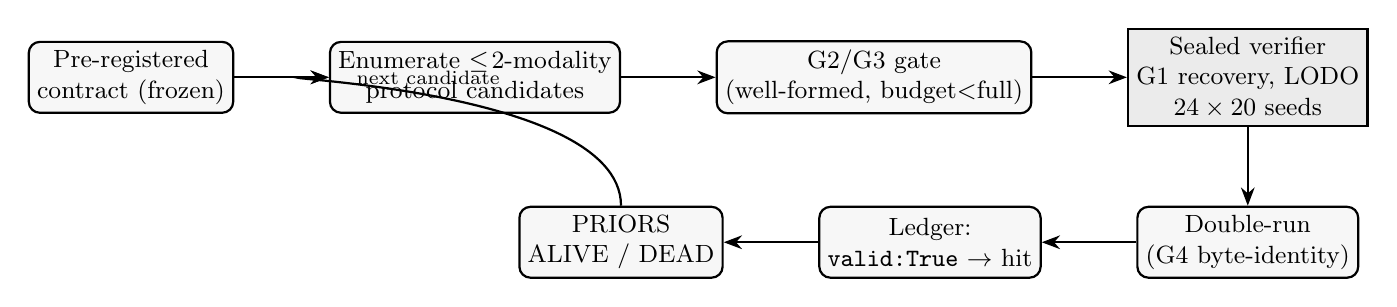
\begin{tikzpicture}[
  node distance=8mm and 12mm,
  box/.style={draw, rounded corners, align=center, minimum height=9mm, inner sep=3pt, font=\small, fill=black!3},
  ora/.style={draw, align=center, minimum height=9mm, inner sep=3pt, font=\small, fill=black!8},
  >={Stealth[]}, thick]
\node[box] (hyp) {Pre-registered\\contract (frozen)};
\node[box, right=of hyp] (enum) {Enumerate $\le\!2$-modality\\protocol candidates};
\node[box, right=of enum] (gate) {G2/G3 gate\\(well-formed, budget$<$full)};
\node[ora, right=of gate] (ver) {Sealed verifier\\G1 recovery, LODO\\$24\times20$ seeds};
\node[box, below=10mm of ver] (dbl) {Double-run\\(G4 byte-identity)};
\node[box, left=of dbl] (ledger) {Ledger:\\\texttt{valid:True} $\to$ hit};
\node[box, left=of ledger] (priors) {PRIORS\\ALIVE / DEAD};
\draw[->] (hyp) -- (enum);
\draw[->] (enum) -- (gate);
\draw[->] (gate) -- (ver);
\draw[->] (ver) -- (dbl);
\draw[->] (dbl) -- (ledger);
\draw[->] (ledger) -- (priors);
\draw[->] (priors.north) to[out=90,in=180] node[above,font=\scriptsize]{next candidate} (enum.west);
\end{tikzpicture}
\caption{Harness loop for this campaign. A frozen contract fixes the objective and gates; the searcher enumerates candidate protocols and calls the blinded sealed verifier; a claimed hit becomes a ledger fact only after a byte-identical double-run (G4). Beliefs (ALIVE/DEAD) carry the verdict id as provenance.}
\label{fig:loop}
\end{figure}

\section{Results}

We report search evidence by run id: run~1 is \textbf{SEARCH-1}, run~2 is \textbf{SEARCH-2}. Two islands ran per run (lenses \textsc{small-first} and \textsc{structure-first}).

\subsection{Setup diagnostics: which modalities are load-bearing}

Before any candidate was graded, the pre-search leverage check quantified how many millivolts dropping each modality moves the full-protocol answer across the grid (Table~\ref{tab:leverage}). TRPL moves it by $0.31\mV$, below the $10\mV$ bar, hence \emph{non-load-bearing by construction} for the implied-$\Voc$ scalar. This is expected, not a discovered shortcut: TRPL's PLQE route is a noisier ($\sigma=0.20$) duplicate of SRPL's direct route ($\sigma=0.03$), so for the $\Voc$ number it is redundant. SRPL ($20.06\mV$) and transmission ($47.25\mV$) are both load-bearing. The dress rehearsal passed ($<10^{-6}\,\mathrm{V}$ residual, referee faithful) and the full-protocol seed scatter was below the $10\mV$ tolerance (not ill-posed), so the bar is achievable in principle and grading was authorized.

\begin{table}[t]
\centering
\caption{Setup leverage (SEARCH-1/SEARCH-2): millivolts by which dropping each modality moves the full-protocol implied $\Voc$, worst-case over the $24\times20$ grid. Load-bearing $=$ leverage $>10\mV$.}
\label{tab:leverage}
\begin{tabular}{lrl}
\toprule
Dropped modality & Leverage (mV) & Load-bearing? \\
\midrule
Transmission & $47.25$ & yes \\
SRPL         & $20.06$ & yes \\
TRPL         & $0.31$  & no (redundant for the $\Voc$ scalar) \\
\bottomrule
\end{tabular}
\end{table}

\subsection{The reduction exists: three certified passers}

Exhaustive enumeration of the single-config protocols across the six size-$\le 2$ subsets found that every certified passer lies in the single subset $\{$SRPL, transmission$\}$, at transmission window $20$~ms and SRPL photon dose $\gtrsim 12.5$. The ledger records three double-run-certified hits (SEARCH-2), listed in Table~\ref{tab:hits}. All three Pareto-dominate the full protocol's $(220,201)$ budget; the cheapest, H3, recovers the full implied $\Voc$ to $9.13\mV$ worst-case while cutting acquisition time by $68\%$ ($220\to70\,$ms) and photon dose by $93\%$ ($201\to13.5$).

\begin{table}[t]
\centering
\caption{Certified passers (SEARCH-2), all in the $\{$SRPL, transmission$\}$ subset with transmission at $20$~ms. Budgets are computed by the pinned accounting; verdicts and the H3 worst-case error are sealed-verifier outputs. All three satisfy G1 ($\le 10\mV$), G2, and G3 (strict Pareto-dominance of the full $(220,201)$ budget).}
\label{tab:hits}
\begin{tabular}{llrrrl}
\toprule
ID & SRPL config & Time (ms) & Dose & Worst-case & Verdict \\
\midrule
Full (ref.) & $f{=}1.0,\ 100$ ms $+$ TRPL $+$ trans & $220$ & $201.0$ &, & (reference) \\
H1 & $f{=}1.0,\ 100$ ms & $120$ & $101.0$ & $\le 9.13\mV$ & \texttt{valid:True} \\
H2 & $f{=}1.0,\ 50$ ms  & $70$  & $51.0$  & $\le 9.13\mV$ & \texttt{valid:True} \\
H3 & $f{=}0.25,\ 50$ ms & $70$  & $13.5$  & $9.13\mV$     & \texttt{valid:True} \\
\bottomrule
\end{tabular}
\end{table}

The worst-case recovery error is governed by SRPL photon dose (fluence and window enter only through their product) and by transmission dose; it is monotone decreasing in SRPL dose. H3 sits just inside the bar at SRPL dose $12.5$ (fluence $0.25\times50$~ms; its total budgeted dose $13.5$ adds the $1.0$ from transmission); H1 and H2 carry strictly more SRPL dose ($100$ and $50$) and therefore clear the bar by a larger margin (worst-case $\le$ H3's $9.13\mV$; the near-miss series below establishes monotonicity, so ``$\le$'' is a sound bound). Figure~\ref{fig:cliff} plots the recovery cliff.

\subsection{The complementary negative: dropping SRPL or transmission fails}
\label{sec:negative}

Enumeration also \emph{certifies the negative over the single-config space}. Every single-config protocol that drops a load-bearing modality misses the $10\mV$ bar (Table~\ref{tab:frontier}). We then bound what multi-config repeats (not exhaustively graded) could rescue.

\paragraph{Dropping transmission (airtight against repeats).} Removing transmission forces the bandgap, thickness, and Urbach energy onto coarse LODO priors and pushes the error above $47\mV$ (e.g. $64.22\mV$ for the single-config SRPL$(0.25,50\text{ms})$+TRPL). No amount of PL repetition changes this: neither SRPL nor TRPL measures $E_g$ or $d$ at any dose (\S\ref{sec:forward}), so no multi-config PL protocol supplies the absorption-edge information transmission carries. The transmission-dropping negative therefore holds for the full contract space, not only single configs.

\paragraph{Dropping SRPL (single-config floor $20.06\mV$; repeats bounded, not graded).} Keeping only TRPL's indirect PLQE, the single-config error floors at $20.06\mV$ (exactly SRPL's leverage) because the indirect route ($\sigma=0.20$) is structurally too imprecise to replace the direct one ($\sigma=0.03$). TRPL repeats \emph{do} lower the indirect-PLQE variance as $\sqrt{\text{dose}}$, so multi-config drop-SRPL protocols are the one family the single-config enumeration does not settle. Within the $(220,201)$ budget the achievable dose increase is bounded (roughly a doubling of TRPL dose while keeping transmission at $5$~ms), which narrows but (on a variance-scaling estimate) does not close the gap to the SRPL-direct route below $10\mV$. We report this as an \emph{argued} bound, not a graded certification, and scope the drop-SRPL negative to the single-config protocols we actually enumerated; exhaustively grading the multi-config drop-SRPL family is the natural next check.

\paragraph{Single-modality and near-misses.} Transmission-only carries no PLQE information at all and misses by $58.02\mV$. The tightest near-misses are all inside the winning subset, at the SRPL-dose cliff (dose $10\to10.33\mV$, just $0.33\mV$ over) or under transmission-dose starvation (transmission at $5$~ms $\to 13.24\mV$ unless rescued by high SRPL dose). Figure~\ref{fig:budget} places the passers and the frontier against the full-protocol budget.

\begin{table}[t]
\centering
\caption{Near-miss frontier (SEARCH-1/SEARCH-2): the best failing single-config protocols and why they miss. Budgets by the pinned accounting; worst-case errors are sealed-verifier outputs. ``Drop X'' means modality X is absent (its quantities come from LODO priors).}
\label{tab:frontier}
\begin{tabular}{llrrl}
\toprule
Protocol & Family & Time & Dose & Worst-case (mV) \\
\midrule
SRPL$(0.1,100)$ $+$ trans$(20)$   & keep both, low SRPL dose $10$ & $120$ & $11.0$  & $10.33$ \\
SRPL$(1.0,10)$ $+$ trans$(20)$    & keep both, low SRPL dose $10$ & $30$  & $11.0$  & $10.33$ \\
SRPL$(0.1,50)$ $+$ trans$(20)$    & keep both, SRPL dose $5$      & $70$  & $6.0$   & $14.26$ \\
SRPL$(0.25,100)$ $+$ trans$(5)$   & keep both, trans starved      & $105$ & $25.25$ & $13.24$ \\
TRPL$(1.0,100\text{ns})$ $+$ trans$(20)$ & drop SRPL              & $120$ & $101.0$ & $20.06$ \\
SRPL$(0.25,50)$ $+$ TRPL$(1.0,100\text{ns})$ & drop transmission & $150$ & $112.5$ & $64.22$ \\
Transmission$(5)$ only            & drop SRPL \& TRPL             & $5$   & $0.25$  & $58.02$ \\
\bottomrule
\end{tabular}
\end{table}

\begin{figure}[t]
\centering
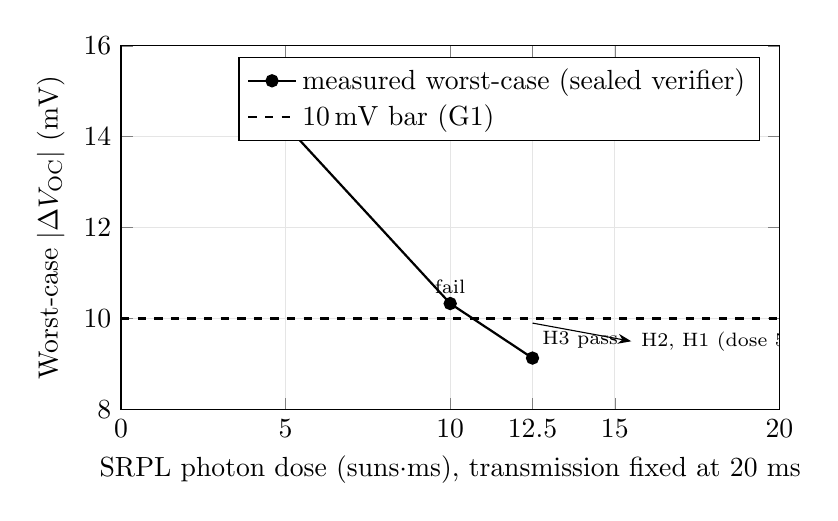
\begin{tikzpicture}
\begin{axis}[
  width=0.82\textwidth, height=6.2cm,
  xlabel={SRPL photon dose (suns$\cdot$ms), transmission fixed at $20$~ms},
  ylabel={Worst-case $|\Delta\Voc|$ (mV)},
  xmin=0, xmax=20, ymin=8, ymax=16,
  xtick={0,5,10,12.5,15,20},
  ytick={8,10,12,14,16},
  legend pos=north east, legend cell align=left,
  grid=both, grid style={black!10},
]
\addplot[thick, mark=*, mark size=2pt] coordinates {(5,14.26) (10,10.33) (12.5,9.13)};
\addlegendentry{measured worst-case (sealed verifier)}
\addplot[dashed, thick, domain=0:20] {10};
\addlegendentry{$10\mV$ bar (G1)}
\node[anchor=south west, font=\scriptsize] at (axis cs:12.5,9.13) {H3 pass};
\node[anchor=south, font=\scriptsize] at (axis cs:10,10.33) {fail};
\draw[->, >=Stealth] (axis cs:12.5,9.9) -- (axis cs:15.5,9.5) node[right, font=\scriptsize] {H2, H1 (dose 50, 100)};
\end{axis}
\end{tikzpicture}
\caption{Recovery cliff for the winning $\{$SRPL, transmission$\}$ subset with transmission fixed at $20$~ms. The horizontal axis is \emph{SRPL} photon dose (fluence $\times$ window); worst-case error over the $24\times20$ grid falls monotonically with it and crosses the $10\mV$ bar between SRPL dose $10$ (fail, $10.33\mV$) and SRPL dose $12.5$ (H3 pass, $9.13\mV$; H3's total budgeted dose is $13.5$ including the transmission contribution). H1 and H2 carry more SRPL dose and pass with larger margin. Points are sealed-verifier outputs (SEARCH-2).}
\label{fig:cliff}
\end{figure}

\begin{figure}[t]
\centering
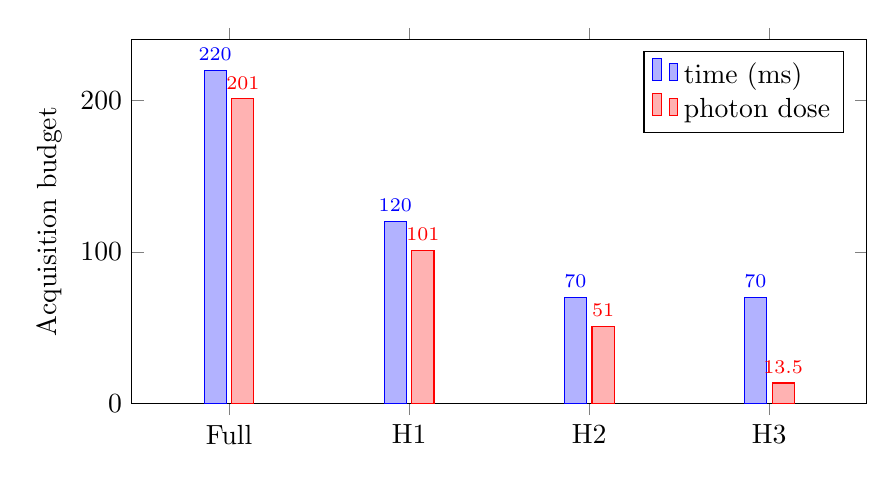
\begin{tikzpicture}
\begin{axis}[
  width=0.9\textwidth, height=6.2cm,
  ybar, bar width=8pt,
  symbolic x coords={Full, H1, H2, H3},
  xtick=data,
  ymin=0, ymax=240,
  ylabel={Acquisition budget},
  legend pos=north east, legend cell align=left,
  nodes near coords, every node near coord/.append style={font=\scriptsize},
  enlarge x limits=0.18,
]
\addplot coordinates {(Full,220) (H1,120) (H2,70) (H3,70)};
\addlegendentry{time (ms)}
\addplot coordinates {(Full,201) (H1,101) (H2,51) (H3,13.5)};
\addlegendentry{photon dose}
\end{axis}
\end{tikzpicture}
\caption{Acquisition budget of the full three-measurement protocol versus the three certified two-measurement passers (SEARCH-2). Every passer strictly Pareto-dominates the full protocol (G3). The dose-frugal H3 cuts time by $68\%$ and photon dose by $93\%$ (total budgeted dose $201\to13.5$).}
\label{fig:budget}
\end{figure}

\subsection{Referee integrity: run 1 rejected, root-caused, re-certified}
\label{sec:integrity}

The determinism gate did real work. In SEARCH-1, three $\{$SRPL, transmission$\}$ candidates were \emph{claimed} but failed the byte-identical double-run and were correctly recorded as non-hits ($0$ verified of $3$ claimed; run stats: $2$ islands, $229$ candidates, $7$ near-misses). Root cause was a fusion routine returning \texttt{NaN} at the infinite-dose limit exercised by the dress rehearsal (equal floored weights over zero noise). A reviewer patched the verifier source (floored the fusion $\sigma$; the code also received a NumPy \texttt{trapezoid} rename and a candidate-parse fallback, all $2026$-$08$-$26$). The patch touches only the infinite-dose dress-rehearsal path: the finite-dose G1 grading path never reaches the floor, so the graded worst-case values are unchanged, for identical candidates the finite-dose numbers are byte-identical across runs (e.g. SRPL$(0.1,100)$+trans$(20)=10.33\mV$ in both runs; drop-SRPL $=20.06\mV$ in both). What changed is the run-1 verdicts' \emph{byte-identity} at the dress-rehearsal stage (fail$\to$pass), not any finite-dose G1 value. In SEARCH-2 the same three protocols verified byte-identically and entered the ledger as hits ($3$ verified of $3$ claimed; $2$ islands, $161$ candidates, $5$ near-misses). We report this because it is the intended behaviour: a self-reported ``hit'' that cannot survive a double-run is not a hit, and the referee's own integrity gate caught a referee bug before any result was accepted. The public contract, the grid, and the gates were never edited; the SHA that pins the contract is constant across the whole campaign.

\section{Discussion}

For this pinned forward model, the implied-$\Voc$ scalar needs a \emph{direct} PLQE measurement and an \emph{absorption-edge} measurement, and nothing else. SRPL supplies the first; transmission supplies the second (and the thickness and Urbach inputs to the radiative term). TRPL's contribution (a second, noisier PLQE estimate) is washed out by inverse-variance fusion and moves the answer by $0.31\mV$. The practical reading, \emph{within the model's scope}, is that a two-measurement workflow (one steady-state PL, one transmission) reproduces the three-measurement implied $\Voc$ to under $10\mV$ at a fraction of the acquisition cost, and that the remaining budget is best spent on SRPL dose (the binding precision) rather than on TRPL.

Two boundaries of the claim deserve emphasis. First, the cliff is set by \emph{information}, not by any single tunable: worst-case error depends on SRPL and transmission \emph{dose}, so equal-dose single configurations grade identically, and the passing threshold is a dose ($\sim 11$--$13$ suns$\cdot$ms of SRPL), not a particular fluence--window pair. Second, the negative is nearly as informative as the positive, with one honest boundary: dropping transmission provably fails for the entire contract space (PL carries no absorption-edge information at any dose), and dropping SRPL fails for every single-config protocol we graded, with a variance-scaling argument (not a brute-force certification) that budget-bounded TRPL repeats do not rescue it. So the strong reading, ``TRPL is the only droppable modality,'' is certified for single configs and argued for repeats; closing the multi-config drop-SRPL case by enumeration would upgrade it to fully certified.

\paragraph{Outlook.} This is a model-based result. The structural claim, that implied $\Voc$ is fixed by one absorption-edge measurement and one direct PL-yield measurement while time-resolved PL is only a noisier second route to the same yield, is physically motivated and stable across the noise range we probed; but the quantitative numbers are outputs of an uncalibrated forward model. The natural next step is empirical validation: fit the forward model to a real paired-measurement dataset (for example the $>100$-device set characterized in Louks \emph{et al.}~\cite{louks2025}) and rerun the same sealed search on measured SRPL, TRPL, and transmission data, testing whether a two-measurement protocol reproduces the full protocol's implied $\Voc$ to the same tolerance on real samples.

\section{Limitations}

\begin{itemize}
\item \textbf{Not empirically validated.} Every number here is computed against a synthetic forward model; none has been tested against real measurements. The result is a quantified hypothesis about the physical system, not an experimental finding. Validation on a real paired-measurement dataset is the natural next step (see the Outlook above).
\item \textbf{The TRPL result is structural, not a search discovery.} TRPL maps to a single quantity (PLQE) that SRPL measures directly, so TRPL can never be uniquely necessary for the implied-$\Voc$ scalar; its $0.31\mV$ leverage is set by the quantity map and is essentially independent of the device values, and the winning protocol's worst-case error equals that leverage. The contribution is the exhaustive, certified confirmation of this, and of the complementary necessity of SRPL and transmission, not a discovery that TRPL happens to be redundant.
\item \textbf{SRPL's necessity is the least robust to the bar.} Transmission ($47\mV$ leverage) and TRPL ($0.3\mV$) sit far from the $10\mV$ threshold, but SRPL's $20\mV$ clears it by only $2\times$: at a ${\sim}25\mV$ tolerance SRPL would flip to non-load-bearing and the two-measurement subset would no longer be unique. The conclusion is a statement at the $10\mV$ bar, and SRPL's necessity is the part most sensitive to it.
\item \textbf{All measurement routes are unbiased by construction.} Each modality reports the true quantity plus zero-mean noise, so precision-weighted fusion collapses to the most precise route and a redundant route is always free to drop. Real indirect-PLQE reconstruction (the TRPL route) can carry \emph{systematic} inter-route offsets from an assumed injection level or radiative coefficient; a biased route would shift the fused answer and could change which modalities are load-bearing. Zero bias is the assumption that makes redundancy free, and it is the deepest lever behind the result.
\item \textbf{Scope is the model's own output, not device $\Voc$.} G1 grades recovery of the full protocol's \emph{implied} $\Voc$ under one pinned forward model. It says nothing about agreement with a device's measured JV $\Voc$; the ${\sim}170\mV$ implied-to-contacted offset in real perovskite stacks~\cite{louks2025} is out of scope and is identical for both protocols.
\item \textbf{Synthetic grid, pinned physics.} The $24$-device grid (a single random draw), the detailed-balance model, the noise scalings ($\sigma_{\mathrm{PLQE}}^{\mathrm{SRPL}}=0.03$, $\sigma_{\mathrm{PLQE}}^{\mathrm{TRPL}}=0.20$, $\pm2\mV$ on $E_g$, etc.), and the budget accounting are all fixed by the contract. Conclusions hold for this model and this grid draw. A grid widened beyond the published batch spread, a different noise floor, or a TRPL route with materially better precision could change which modalities are load-bearing; the leverage check is the guard that would flag it. The cheapest-passer status of H3 (which sits $0.87\mV$ under the bar) and the exact dose cliff are properties of this grid realization, not just the parameter box.
\item \textbf{The multi-config drop-SRPL family is argued, not graded.} The certified negative is exhaustive over single-config protocols. Transmission-dropping is additionally airtight against repeats; SRPL-dropping is bounded by a variance-scaling argument but not brute-forced over multi-config TRPL repeats. The ``exists'' headline does not depend on this; the ``only droppable modality'' reading does, and is scoped accordingly.
\item \textbf{Tolerance and grid are pre-registered, not optimized.} The $10\mV$ bar and the certification seeds ($1000$--$1019$) were frozen before grading. The result is a statement at that bar; it does not certify recovery at, say, $5\mV$.
\item \textbf{Existence, not global cost-optimality.} We certify that passers exist in exactly one subset and report the dose-minimal recorded hit. We do not claim H3 is the unique cost-optimal protocol across every budget metric; other passers in the family trade time against dose.
\end{itemize}

\section{AI-contribution statement}

The authors are responsible for this work and have verified its claims. All quantitative results are outputs of a sealed, deterministic verifier whose contract was frozen before grading; the authors reviewed the verifier, the frozen contract, and every recorded verdict, and re-ran the oracle to confirm the reported numbers. An automated multi-agent research harness (Anthropic Claude models) executed the mechanical steps under human direction: enumerating candidate protocols, calling the blinded verifier, logging verdicts to an append-only ledger, and drafting this manuscript from that ledger. The harness proposed no result that a human did not verify against the sealed oracle, and no AI system is an author. Numbers stated as measured are verifier verdicts; numbers stated as budgets are computed by the pinned accounting and were checked against the contract.

\section{Code and data availability}

The reproduction repository \texttt{github.com/oharalabsai/voc-minimal-subset-repro} contains the frozen contract, the sealed verifier (\texttt{verifier.py}), including the forward model, the $24$-device grid generator, the noise model, the budget accounting, and the dress-rehearsal and pre-search integrity checks, every scored candidate with its verdict, and the append-only ledger. Because this is a closed search campaign, the verifier itself is published, so every verdict in Tables~\ref{tab:leverage}--\ref{tab:frontier} and Figures~\ref{fig:cliff}--\ref{fig:budget} can be recomputed byte-for-byte, and the multi-config drop-SRPL family flagged in \S\ref{sec:negative} can be graded directly against the same oracle. A one-command \texttt{reproduce.py} (plus \texttt{requirements.txt}) re-runs the integrity checks and re-verifies every certified hit from the ledger.

\bibliographystyle{unsrt}
\bibliography{references}

\end{document}
